\documentclass[screen]{beamer}
\usepackage[T1]{fontenc}
\usepackage[utf8]{inputenc}
\usetheme{ntnubokmaal}
\usepackage{wasysym}
\usepackage{color}

\title[Status bacon]{Status for Futhark, MiA 2011}
\subtitle{Steking av bacon i mikrobølgeovn}
\author[Futhark]{Å. Ervik, K. H. Skrede, T. S. Solberg, P. Vo, J. Johnsen}
\institute[NTNU]{Eksperter i Team, NTNU}
\setbeamertemplate{footline}[ntnu theme nologo]
\date{30.03.2011}

\newcommand{\gv}[1]{\ensuremath{\mbox{\boldmath$ #1 $}}}
\renewcommand{\div}[1]{\gv{\nabla} \cdot #1} % for divergence
\newcounter{saveenumi}
%\newcommand{\labelitemi}{$\bullet$}
\newcommand{\checktick}{\textcolor{green}{\checked}}

\begin{document}
\ntnutitlepage

\begin{frame}
  \frametitle{Problemstilling}
  \begin{center}
  \begin{itemize}  
  \item[$\bullet$] Hvordan kan steking av bacon i en mikrobølgeovn modelleres matematisk? 
  \item[$\bullet$] Hvordan vil fett-, vann- og saltinnhold påvirke stekingen, og hvilken effekt er optimal? 
  \end{itemize}
  \end{center}
\end{frame}

\begin{frame}
  \frametitle{Planen}
  \begin{enumerate}
  \item Varme
  \item Massetransport
  \item Nøyaktige grensebetingelser for mikrobølgeovn
    \setcounter{saveenumi}{\theenumi}
\end{enumerate}
    \hline
\begin{enumerate}
    \setcounter{enumi}{\thesaveenumi}
  \item Elektromagnetiske grensebetingelser
  \item App - redusert modell
  \end{enumerate}
\end{frame}

\begin{frame}
  \frametitle{Status numerikk}
  \begin{enumerate}
  \item[\checktick] Varme
  \item[2.] Massetransport
  \item[\checktick] Nøyaktige grensebetingelser for mikrobølgeovn
\end{enumerate}
    \hline
\begin{enumerate}
  \item[4.] Elektromagnetiske grensebetingelser
  \item[5.] App - redusert modell
  \end{enumerate}
\end{frame}

\begin{frame}
  \frametitle{Status eksperimenter}
    \begin{center}
      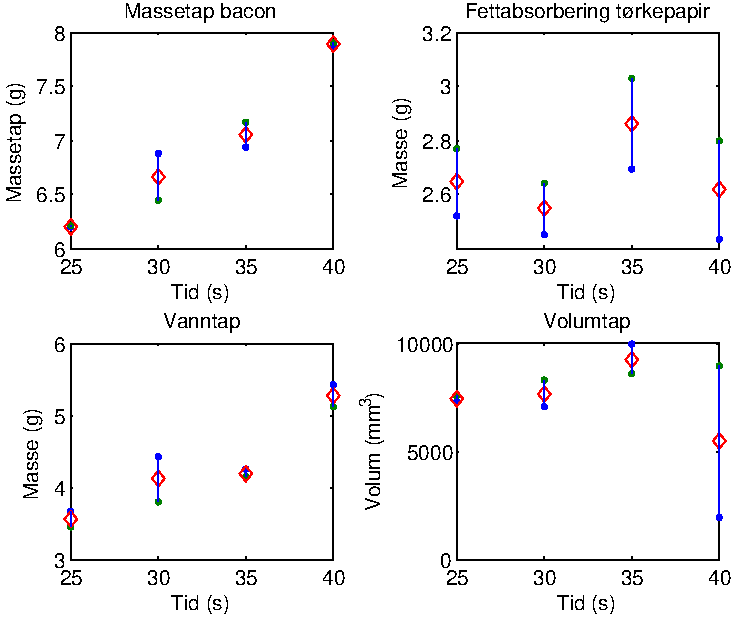
\includegraphics[width=0.7\linewidth]{eksperiment.pdf}
    \end{center}
\end{frame}

\begin{frame}
  \frametitle{Gruppestruktur}
  \begin{itemize}
    \item[$\bullet$] Flat struktur med situasjonsbetinget ledelse
	\begin{quote}{
	  \tiny
	Når det skal tas en avgjørelse om valg av numerisk modell, er det
	numerikerne som er sjef.}
	\end{quote}
    \item[$\bullet$] Dynamisk arbeidsfordeling 
      \begin{quote}{
	\tiny
	Ressursene brukes der det trengs. Da vi hadde problemer i numerikken og
	Knut Halvor trengte hjelp, bidro de andre medlemmene til å debugge
	koden.}
	\end{quote}
    \item[$\bullet$] Godt teamarbeid når problemer oppstår
      \begin{quote}{
	\tiny
        Det blir ikke desperasjon når vi treffer på et problem, gruppa er
	løsningsorientert og tilpasningsdyktig.}
      \end{quote}
  \end{itemize}
\end{frame}

\begin{frame}
  \frametitle{Kommunikasjon}
  \begin{itemize}
    \item[$\bullet$] Gruppa er flink til å kommunisere når noen tar initiativ
      \begin{quote}{
	\tiny
      Kaffepause er et eksempel. Turid er god ordstyrer i de situasjoner der
      det trengs.}
      \end{quote}
    \item[$\bullet$] Kommunikasjon er det området der gruppa har størst forbedringspotensiale
      \begin{quote}{
	\tiny
      Gruppemedlemmene har ikke alltid oversikt over alt de andre gjør.
      Forbedring kan gjøre at gruppa arbeider mer effektivt.}
      \end{quote}
    \item[$\bullet$] Kompenseres delvis ved at man har stort tiltro til de andre gruppemedlemmene
      \begin{quote}{
	\tiny
      Medlemmene i gruppa er trygge på de andre både faglig og personlig, og
      vet at de vil gjøre sitt beste for å få et godt resultat.}
      \end{quote}
  \end{itemize}
\end{frame}

\begin{frame}
  \frametitle{Karakterisering av gruppa}
  \begin{itemize}
    \item[$\bullet$] Gruppa har høy effektivitet og arbeider veldig godt sammen
    \item[$\bullet$] Forklaring:
      \begin{itemize}
	\item gruppa forholder seg saklig til beslutninger som tas
	  \begin{quote}{
	    \tiny
	  beslutningsprosessen i gruppa bidrar til å forsterke vår felles
	  gruppeidentitet - vi presenterer egne meninger, lytter til andres
	  meninger, og finner en felles platform som vi kan jobbe ut ifra.}
	  \end{quote}
	\item stemningen i gruppa er god i utgangspunktet - vi ``klikker''
	  \begin{quote}{
	    \tiny
	  hvorfor klikker vi? felles tankegang, lik humor. Vi er i samme båt.
	  Ingen av oss er selvhøytidlige, så vi har frihet til å være oss selv
	  i gruppa. Vi trenger ikke å holde noe tilbake.}
	  \end{quote}
	\item gruppemedlemmene er motiverte for å produsere et godt resultat
	  \begin{quote}{
	    \tiny
	  medlemmene er fornøyde med beslutningene som har blitt tatt, og alle
	  føler de er en essensiell del av gruppa. engasjement. OK instilling
	  til EiT.}
	  \end{quote}
      \end{itemize}
  \end{itemize}
\end{frame}

\end{document}



